\chapter{Neural Networks}

\section{Feed-Forward Neural Networks}

Feed-forward Neural Networks are described as a graph $G = (V, E)$ where $V$ are the vertices or neurons and $E$ are the edges, that is the connections between neurons. The edges are characterized by a weight $w$ which represents the strength of the connection between two neurons.

A Feed-forward Neural Network is organized in layers which contain a certain number of neurons. The first layer which takes as input the training data is called the input layer and the final layer that gives the output of the network is called the output layer. Between them we will have a certain number of hidden layers. The number of hidden layers and the neurons that each layer contain defines the architecture of the network.

\begin{figure}[h]
    \centering
    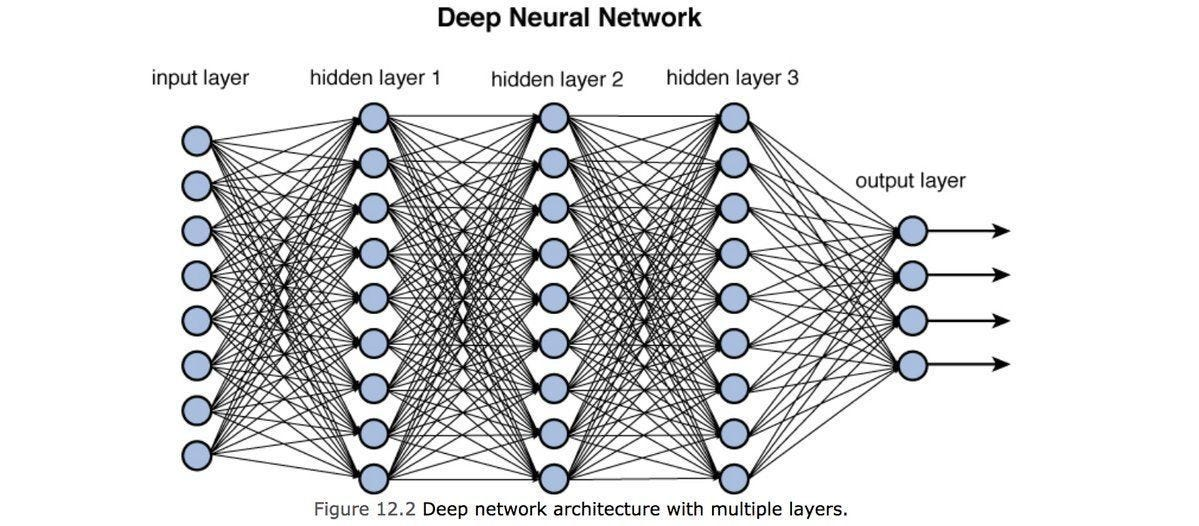
\includegraphics[width=14cm]{Images/feed-forward-nn.jpg}
    \caption{Feed Forward Neural Network architecture}
\end{figure}

\noindent In a Feed-forward Neural Network each neuron is connected to all the neurons of the previous layer, making a fully connected structure. Each neuron then takes as input the sum of the outputs of the connected neurons from the previous layer weighted by the edge weights and it applies to the result a non-linear activation function $\sigma$. The result gives that neuron output which will be used for computing next layer neurons. This process is repeated until reaching the output layer which will give us the network output.

Once the output is obtained we will compare the results with the labels or target of our data in order to calculate the loss. Once we done that we will be able to update the weights of our network and repeat the training process. This is done for $N$ epochs. The goal of the training is therefore learn the weights that best suits our problem.

\newpage
\noindent The simplest kind of Neural Network consists of only the input layer connected to a single unit that operates as the output. This kind of architecture is called a perceptron and is equivalent to simpler Machine Learning models such as logistic regression or Support Vector Machines in that they are only able to model functions which can linearly separate input data.

\begin{figure}[h]
    \centering
    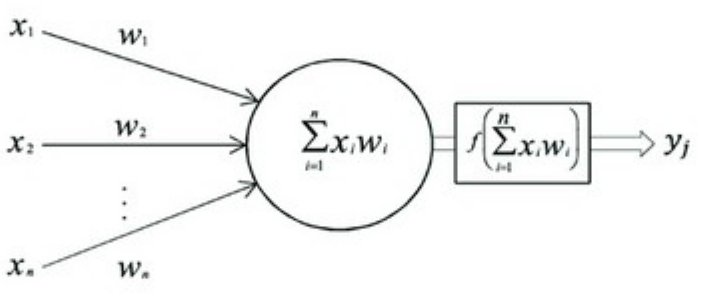
\includegraphics[width=7cm]{Images/perceptron.jpg}
    \caption{The perceptron is the simplest Neural Network architecture}
\end{figure}


\subsection{The Need for Deep Feed-Forward Neural Networks}

Shallow Deep Neural Networks have the same limitations as Machine Learning linear models, as they are not able to work with non-separable data. That's why we introduce non-linearity by means of introducing hidden layers and non-linear activation functions to the output of each neuron of the different hidden layers. This makes the model able to learn non-linear relationships in our data. For example we will only be able to solve the XOR task when we use at least one hidden layer in combination with a non-linear activation function to compute the values of the neurons. 

\begin{figure}[h]
    \centering
    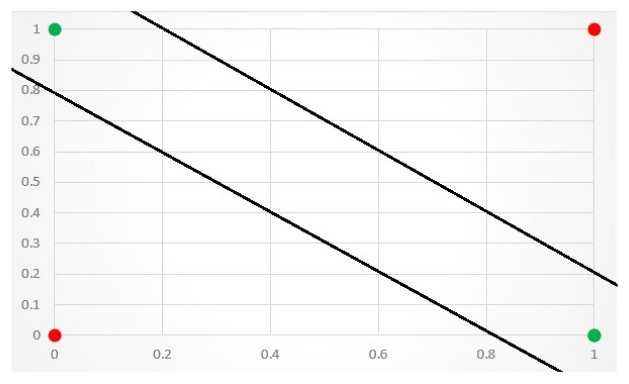
\includegraphics[width=8cm]{Images/xor.jpg}
    \caption{To solve the XOR problem we need to introduce non-linearity.}
    \label{fig:xor}
\end{figure}

\noindent Basically, the idea behind using multiple layers is that complex relations can be broken into simpler functions and combined. This makes our model able to learn more complex patterns in the data which will make it generalise better as the complexity of our model increases. This creates the necessity of using Deep Feed Forward Neural Networks, also called Multi-Layer Perceptrons which are represented as a composition of many different functions if we want to go further than Machine Learning linear models.

$$ f(x) = f^{(3)} \left(f^{(2)}\left(f^{(1)}\right)\right)$$

where $f^{(i)}$ represents the i-th layer.

\newpage
\section{Universal Approximation Theorem}

The Universal Approximation Theorem states that a feed-forward deep neural network with at least one hidden layer and a squashing (non-linear) activation function has the ability to approximate arbitrarily well any continuous function, given enough number of hidden units.

However, having a single hidden layer can require an exponential number of hidden units to approximate a given function with precision. This is why we usually build deeper layers, which will be able to learn more complex representations of our data making multi-layer Neural Networks preferable on practice. In fact, it has been shown that with the same number of parameters deeper networks tend to achieve a better result but at the same time they take more time to train.

Whichever the case there is not guaranteed that the training algorithm will be able to learn the continuous function we are targeting it. This is because the optimization algorithm may not be able to find the value of the parameters that corresponds to the desired function or the training algorithm might choose the wrong function (overfiting). 

\section{Gradient-Based Learning}

The largest difference between the linear Machine Learning models and Neural Networks is that the non-linearity of the network causes most loss functions to become non-convex. This leads to having no guarantee of achieving the global minimum. Therefore we will only be able to reach a local minima which makes our solution sensitive to the starting point.

The choice of the cost function is also an important aspect of the design of a Deep Neural Networks. In most cases, our parametric model defines a distribution $ p( y \vert x, \theta)$ and we simply use the principle of maximum likelihood. This means we use the cross-entropy between the training data and the model’s predictions as the cost function.

$$ J(\theta) = - \mathbb{E}_{x, y \sim p_{data}} \left[  log (p_{model} (y \vert x))  \right] $$

\noindent The specific form of the cost function changes from model to model, depending on the form of $log (p_{model})$. This makes the cost function choice tightly coupled with the choice of the output units.

\subsection{Linear Units for Gaussian Output}

If we set our outputs units to be linear units, this is equivalent to performing a regression task.

$$ \hat{y} = W^{T}h + b $$

\noindent In a regression task where the goal is to model the conditional distribution $p(y | x)$ it is common to use a Gaussian distribution.

$$ p_{model} (y \vert x) = N(y, \hat{y}, I)  $$

\noindent Because performing Maximum Likelihood Estimator in regression is equivalent to minimizing the Mean Squared Error. We will set the cost function as:

$$ J(\theta) = \frac{1}{2} \mathbb{E}_{p \sim p_{data}} \left[ ( y - f(x, \theta) )^2  \right] + constant  $$

using the Mean Squared Error as our cost function.

\newpage
\subsection{Sigmoid Units for Bernoulli Output Distributions}

Instead, in a binary classification problem the probability distribution is given by the Bernoulli distribution. This distribution is defined by a single parameter $\phi$.

$$P(x) = \phi^{x} \left(1 - \phi\right)^{1-x} $$

where  $\phi \in [0 ,1]$ and the Bernoulli distribution can only take two values: $P(x=1)=\phi$~ or ~$P(x=0)=1 - \phi$.

\noindent A Neural Network working in this framework should have as output the probability $\phi$ that given a data sample this belongs to one of the two classes. For example for class 1, this can be written as $P(y=1 | x) $. Since $\phi$ is a probability we should enforce this value to be inside the 0 to 1 range. This can be done by applying a non-linear activation function to the units output $\sigma \left(  w^Th + b \right)$. At the same time we want to ensure that the gradient is not 0 when the model is wrong. A very common choice that fulfills all these requirements is to use a sigmoid activation function which is defined as:

$$ \sigma (x) = \frac{1}{1 + exp(-x)} $$

\noindent We can demonstrate that the sigmoid function is the reasonable choice by operating in the following way. Defining

$$ z = w^T h + b$$

\noindent Then we made the assumption that we can define an unnormalized probability $\hat{P}(y)$ as

$$ \log \left( \hat{P}(y) \right) = yz ~~~ \rightarrow ~~~ \hat{P}(y) = exp(yz) $$

\noindent We can then get the normalize probability $P(y)$ by doing

$$ P(y) = \frac{exp(yz)}{\sum_{y'=0}^{y'=1} exp(y'z)} = \sigma \left( (2y -1)z \right)$$

\noindent Taking into account that the cost function used with maximum likelihood is $-log \left(P(y|x) \right)$ we get:

$$ J(\theta) = - log \left( P(y | x) \right) = - log \left( \sigma \left( (2y -1) z \right) \right) = \zeta \left( \left( 1 -2y \right) z \right)$$

where $\zeta (x) = \log \left( 1 - \exp{(x)} \right)$

\noindent Using sigmoid, saturation will occur when $y=1$ and $z$ is very positive or when $y=0$ and $z$ is very negative. Basically when the model has the right answer that is what we are looking for.

\noindent If we apply other loss loss function like Mean Squared Error, the model will still able to learn but because we are not following the Maximum Likelihood Estimator when operating with a binary classifier it will converge to a worse solution than when using a sigmoid units.

\subsection{Softmax Units for Multinoulli Output Distributions}

To generalize to the case of a discrete variable with $n$ values, we now need to produce an output vector $\hat{y}=[ \hat{y}_0, \hat{y}_1,... , \hat{y}_{n - 1}]$ where $ \hat{y}_i = P(y=i \vert x) $ and we require that:

$$ \forall ~ i ~~ 0 \le \hat{y}_i \le 1   ~~~ \sum_{i} \hat{y}_i = 1 $$

\newpage
\noindent The same approach that worked for the Bernoulli distribution generalizes to the multinoulli distribution. First, a linear layer predicts the un-normalized log probabilities:

$$ z = W^T + b $$

where $ z_i = \log P(y=i \vert x)$. The soft-max function can then exponentiate and normalize $z$ to obtain the desired $\hat{y}$. Formally, the softmax function is given by

$$ softmax (z_i) = \frac{exp(z_i)}{\sum_j exp(z_j)}   $$

\noindent As with the logistic sigmoid, the use of the exponential function works very well when training the softmax to output a target value y using maximum log-likelihood. Defining the softmax in terms of the exponential is natural because the log in the log-likelihood can undo the exponential of the softmax:

$$\log softmax (z)_j = z_i - \log \sum_j \exp{(z_j)}  $$

where the first term $z_i$ encourages the model to increase the output of the correct labels and the second term encourages the model to decrease the output of incorrect labels.

\section{Hidden Units}

Contrary to the output units where we choose the activation function following the maximum likelihood estimator principle, in hidden units there is not a way to define these activation functions beforehand. Nevertheless, a good principle is to use ReLU as a default. This is because linear models are the simplest to optimize. As a result ReLU and their variants, that are still non-linear but have a part of the function that behave linearly, are considered the way to go. More complex activation functions like sigmoid or $\tanh (x)$ can learn a more complex representation of the data as the hypothesis space will be bigger but at the same time they tend to overfit more and are more difficult to optimize. In any way, we will need to perform trial an error between a sample of activation functions in our hidden units to choose the one that works best.

